%%%%%%%%%%%%%%%%%%%%%%%%%%%%%%%%%%%%%%%%%%%%%%%%%%%%%%%%%%%%%%%%%%%%%%%%%%%%%%%%%%%%%%%%%%%%%%%%%%%
%%%%%%%%%%%%%%%%%%%%%%%%%%%%%%%%%%%%%%%%%%%%%%%%%%%%%%%%%%%%%%%%%%%%%%%%%%%%%%%%%%%%%%%%%%%%%%%%%%%
\section{Discusi\'on}

Como se mencion\'o en la secci\'on de hip\'otesis, este trabajo pare del supuesto en que los
sujetos con PDC presentan con mayor probabilidad estacionariedad d\'ebil en sus registros de EEG.
Esta idea fue sugerida por Cohen \cite{Cohen77}, quien a su vez se refiere a trabajos anteriores
sobre regularidad estad\'stica --estacionariedad y normalidad-- sobre registros de 
EEG \cite{McEwen75,Sugimoto78,Kawabata73}. 
Si bien en estos primeros estudios se palpa la posibilidad de que los registros de EEG fueran
ruido de alg\'un tipo, esta idea se ha probado \'erronea en estudios m\'as recientes 
\cite{Klonowski09}.

Cabe entonces mencionar una segunda justificaci\'on, un poco m\'as arbitraria y personal, sobre
las hip\'otesis de este trabajo: en el trabajo de Valeria [no se como citarlo] se describen
diferencias significativas entre los registros de PSG en adultos mayores con y sin PDC,
refiri\'endose al exponente de Hurst ($H_\alpha$) estimado.
La cantidad $H_\alpha$, tambi\'en referido como el ''color'' de la se\~nal,
mide la ''fractalidad''\footnote{Este concepto no se
describir\'a en este trabajo, para m\'as informaci\'on ver el trabajo de Valeria} 
de un proceso estoc\'astico y es estimado a trav\'es del
algoritmo Detrended Fluctuation Analysis (DFA); se reporta
que el exponente $H_\alpha$ es menor para registros de PSG en adultos mayores con PSG, y que es
cercano a aqu\'el en el movimiento browniano. 
Luego entonces, cabe preguntarse sobre la naturaleza exacta de las diferencias detectadas en 
el trabajo de Valeria: ¿la se\~nal es ''menos compleja'' o 
s\'olo ''tiene otro color''?
De manera concreta, en este trabajo se ha hipotetizado sobre la primera opci\'on.

En cierto modo, se ha aportado evidencias suficientes para decir que no hay cambios significativos
en la porci\'on de tiempo durante la cual el registro de PSG se comporta de manera ''simple''
--es PE. Esto puede interpretarse como que --quiz\'a-- los mecanismos afectados durante el PDC no 
provocan que la se\~nal se vuelva m\'as simple desde el punto de vista estad\'istico

Cabe un comentario sobre c\'omo la evidencia exhibe al PSG como se\~nales no-estacionarias
por una porci\'on muy prque\~na de tiempo; luego, no es adecuado analizarla con m\'etodos que
supongan estacionariedad. M\'as a\'un este comentario aplica para individuos con y sin PDC, y
se acent\'ua m\'as en individuos con problemas adicionales.

\subsubsection{La inclusi\'on de sujetos}

Con respecto a los sujetos con problemas adicionales, cabe mencionar el caso de FGH


\subsubsection{Estimadores espectrales de ventana}

\subsubsection{Otros usos para las t\'ecnicas utilizadas}


Un primer tratamiento cualitativo que se dio a los resultados obtenidos del test PSR, es su
disposici\'on gr\'afica.
%Una vez se hubo realizado el test para todas las \'epocas consideradas, se dispuso de los 
%resultados de manera gr\'afica  
%como se muestra en la figura \ref{ejemplo1}.
Se coloc\'o en l\'inea horizontal un cuadro blanco por cada
\'epoca PE (negro para \'epocas no-estacionarias);
% seg\'un el 
%el segmento en cuesti\'on halla sido clasi
%segmento referido haya sido clasificado como
%no-estacionario o posiblemente estacionario; 
posteriormente se colocaron verticalmente las
l\'ineas as\'i obtenidas.
% de todos los canales.
Esta disposici\'on gr\'afica pretende ser consistente con las representaciones gr\'aficas
usuales de EEG.
%, tomando en cuanta una escala m\'as amplia de tiempo gracias a que por
%cada \'epoca s\'olo se ha obtenido un dato.
Puede verse en la figura \ref{ejemplo1} un ejemplo de esta disposici\'on gr\'afica, mientras
que el resto de estos gr\'aficos se incluye como anexo.
%Los gr\'aficos as\'i obtenidos se incluyen como anexo.
%como se muestra en la figura \ref{ejemplo1}.

\begin{figure}
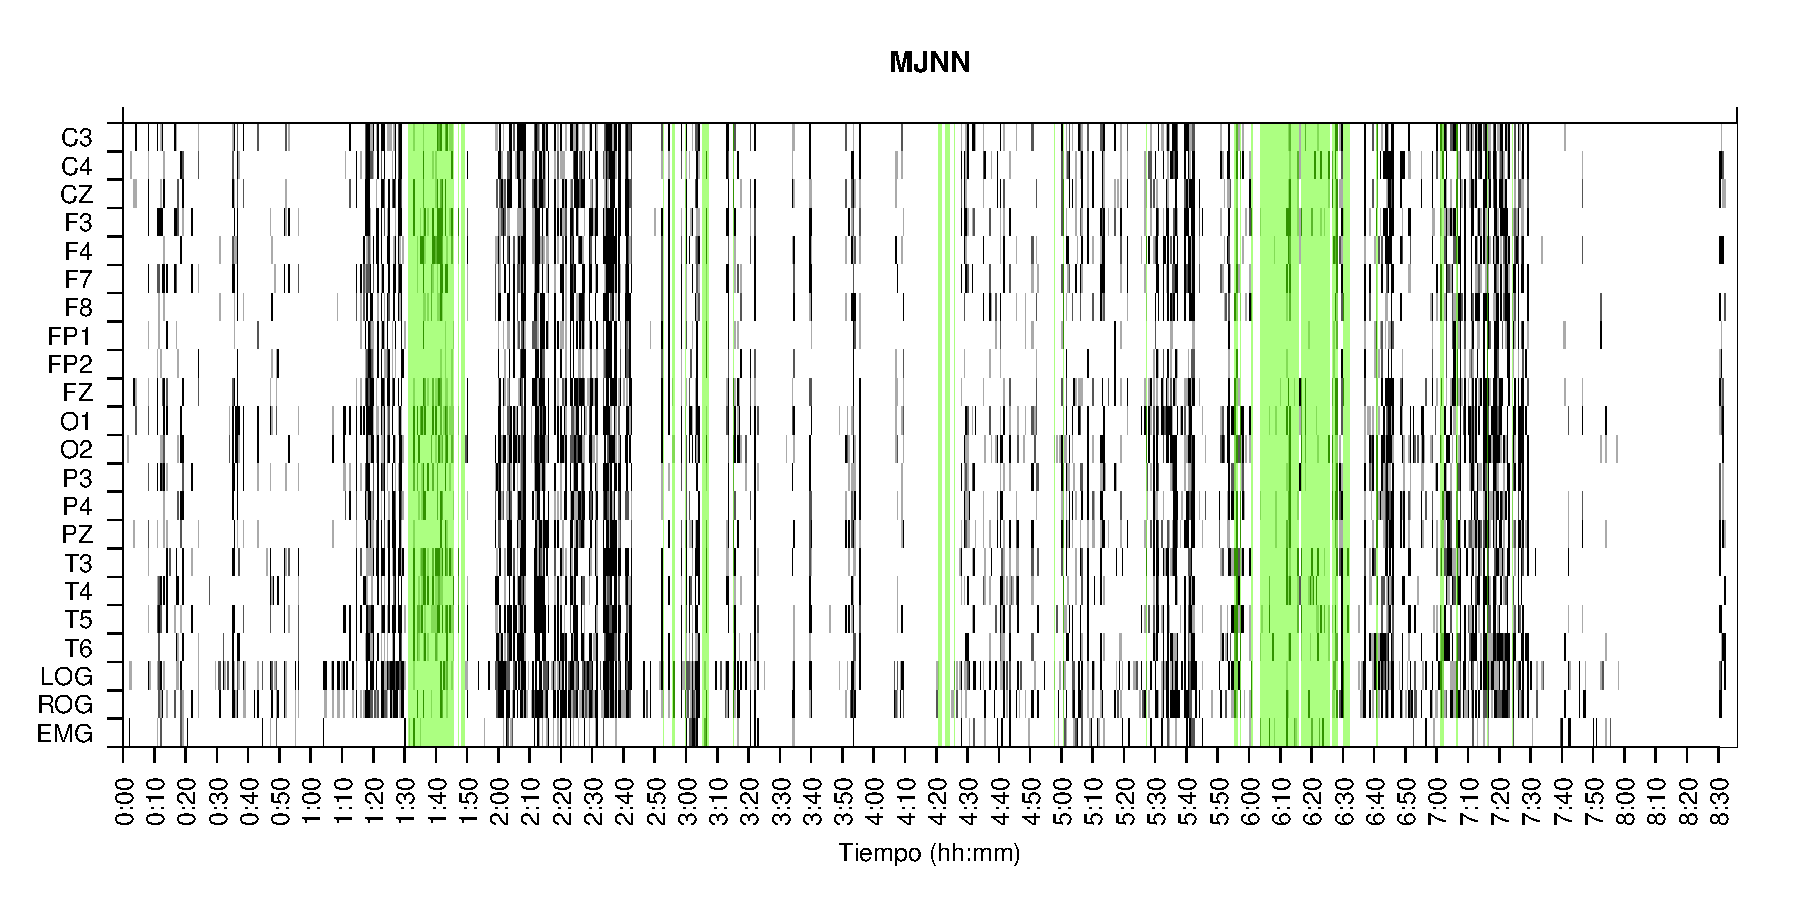
\includegraphics[width=\textwidth]{MJNNVIGILOS_127_mor127_tot1032_esttotal.pdf} 
\caption{Disposici\'on gr\'afica para los resultados del test PSR en el sujeto MJH, 
para 1032 \'epocas de sue\~no y 22 canales. 
En el eje horizontal se muestra el tiempo desde el inicio de registro, en el eje vertical se muestra al 
nombre del canal. 
Se han resaltado con color verde las \'epocas clasificadas como sue\~no MOR (ver texto), que son 127.
Para este gr\'afico se consider\'o con un p-valor cr\'itico de 0.01 para la hip\'otesis
de estacionariedad. Ver texto para m\'as detalles.}
\label{ejemplo1}
\end{figure}

Una debilidad importante de los gr\'aficos as\'i obtenidos es que, si bien muestran patrones 
claros en el tiempo, \'estos no se pueden cuantificar de una manera obvia y se dificulta la
comparaci\'on entre sujetos, raz\'on por la cual se omiti\'on del cuerpo principal del trabajo. 
%Se han inclu\'ido estos resultados porque sus caracter\'isticas 
%sugieren una posible utilizaci\'on para otros fines --en alg\'un trabajo futuro.
Sin embargo, dentro de un mismo sujeto parecen visibles diferencias cualitativas
entre el sue\~no MOR y el resto del sue\~no.

Conviene mencionar que el origen de esta representaci\'on gr\'afica es un intento preeliminar de
fragmentar los an\'alsis de sue\~no MOR en grupos de \'epocas consecutivas en sue\~no MOR ya que,
en general, el sue\~no MOR aparece fragmetnado durante el sue\~no nocturno \cite{CarrilloMora}.
La hip\'otesis de que se podr\'ian definir diferencias que involucraran la componente espacial,
sin embargo, se vio opacada por la dificultad de definir formalmente tales diferencias a modo
que pudieran compararse entre sujetos.
La sugerencia recibida consiste en seguir explorando estos patrones en el tiempo, pero quiz\'a
no con la intenci\'on de detectar deterioro cognitivo sino como apoyo para la identificaci\'on de
diferentes etapas de sue\~no.

%\begin{figure}
%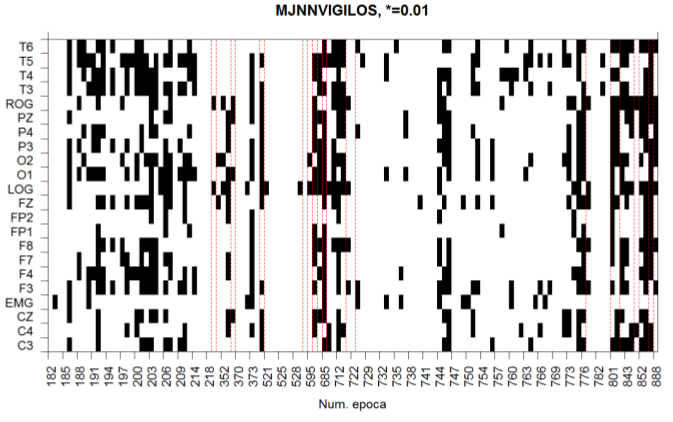
\includegraphics[width=\textwidth]{est02.png} 
%\caption{En este gráfico sólo se ilustran épocas MOR. Las líneas punteadas separan bloques continuos.
%Total de épocas: 1032 , Épocas MOR: 127}
%\label{ejemplo2}
%\end{figure}

%Me siento particularmente orgulloso
%de haber dise\~nado este tipo de gr\'aficos, ya que  organizan datos que ya se ten\'ian
%y dejan la sensaci\'on de portar nueva informaci\'on.

%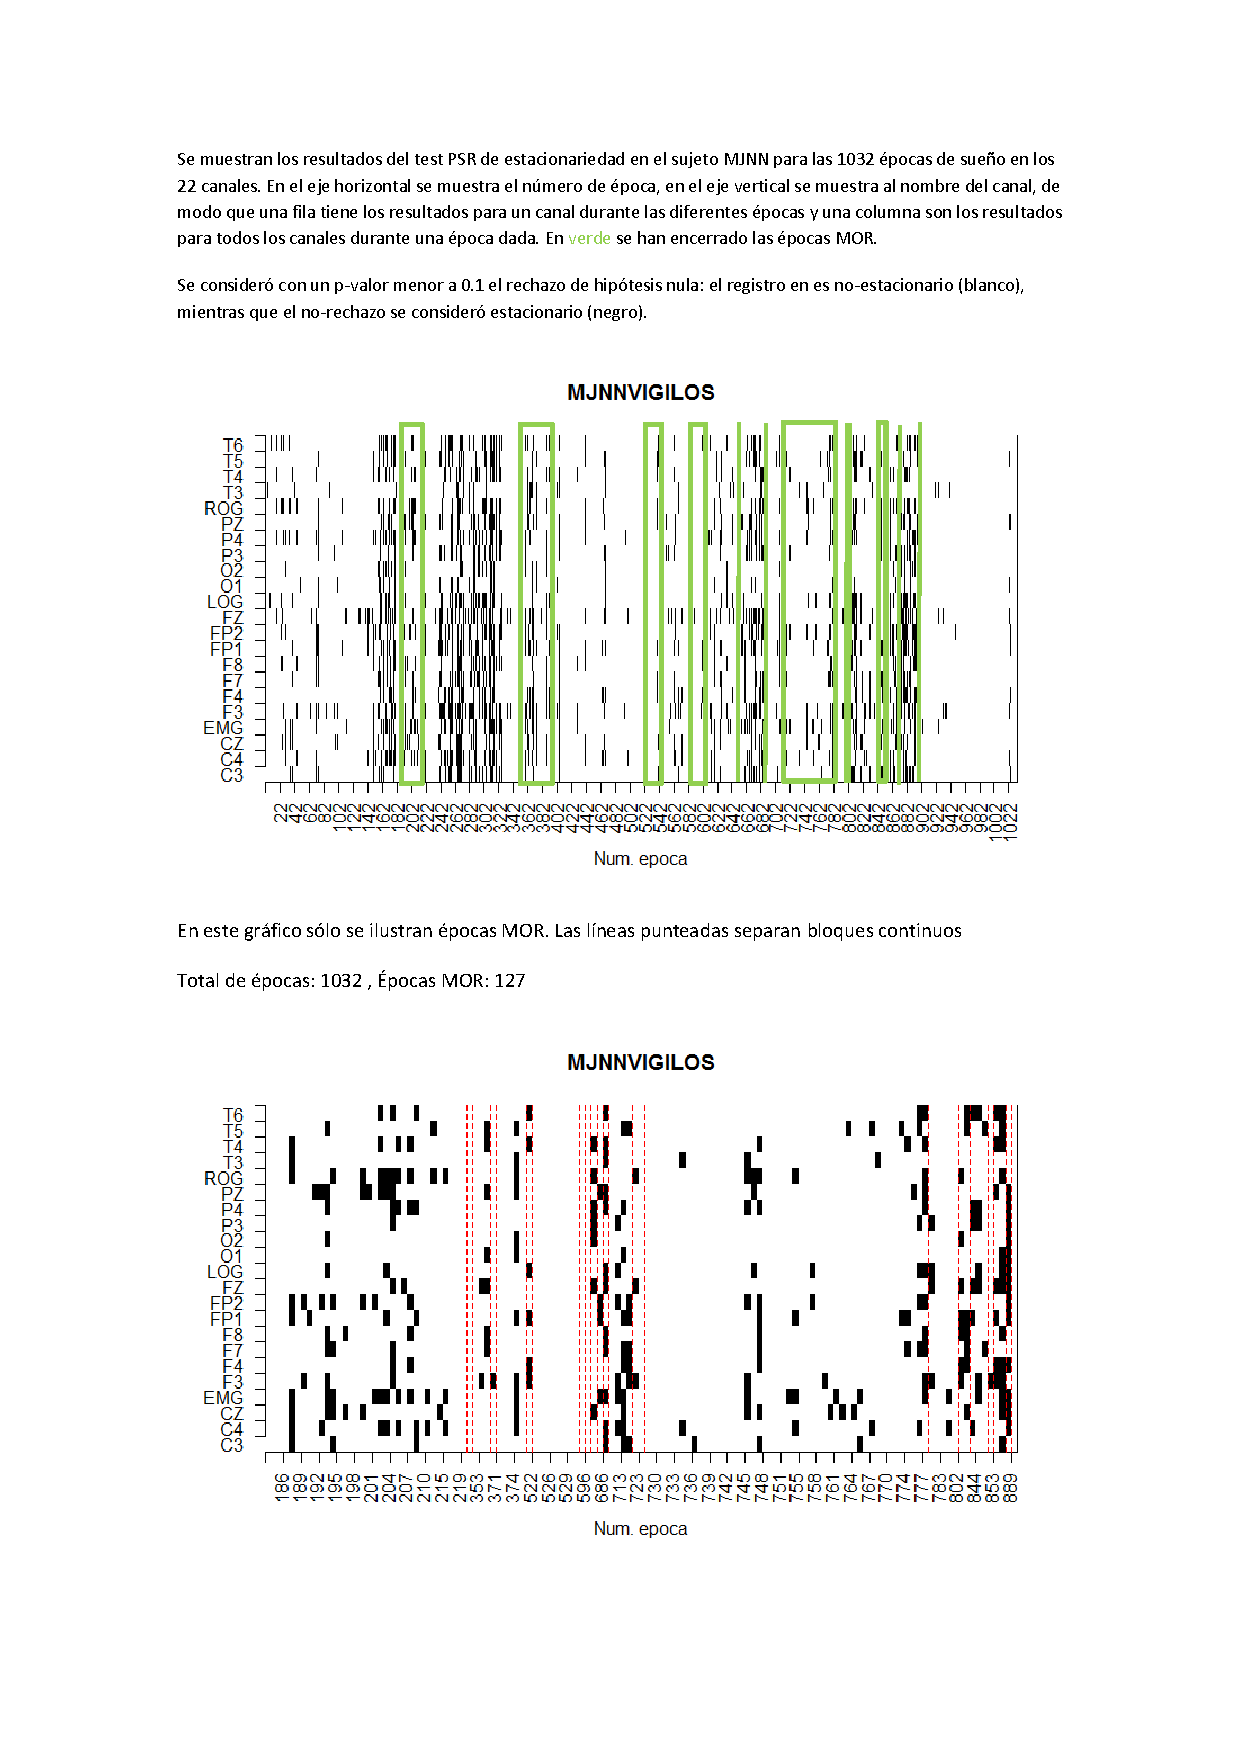
\includepdf[pages={1-},scale=.85]{reporte_de_estacionariedad_170120.pdf}
%
%\afterpage{%
%    \clearpage% Flush earlier floats (otherwise order might not be correct)
%    \thispagestyle{empty}% empty page style (?)
%    \begin{landscape}% Landscape page
%        \centering % Center table
%        \begin{figure}
%            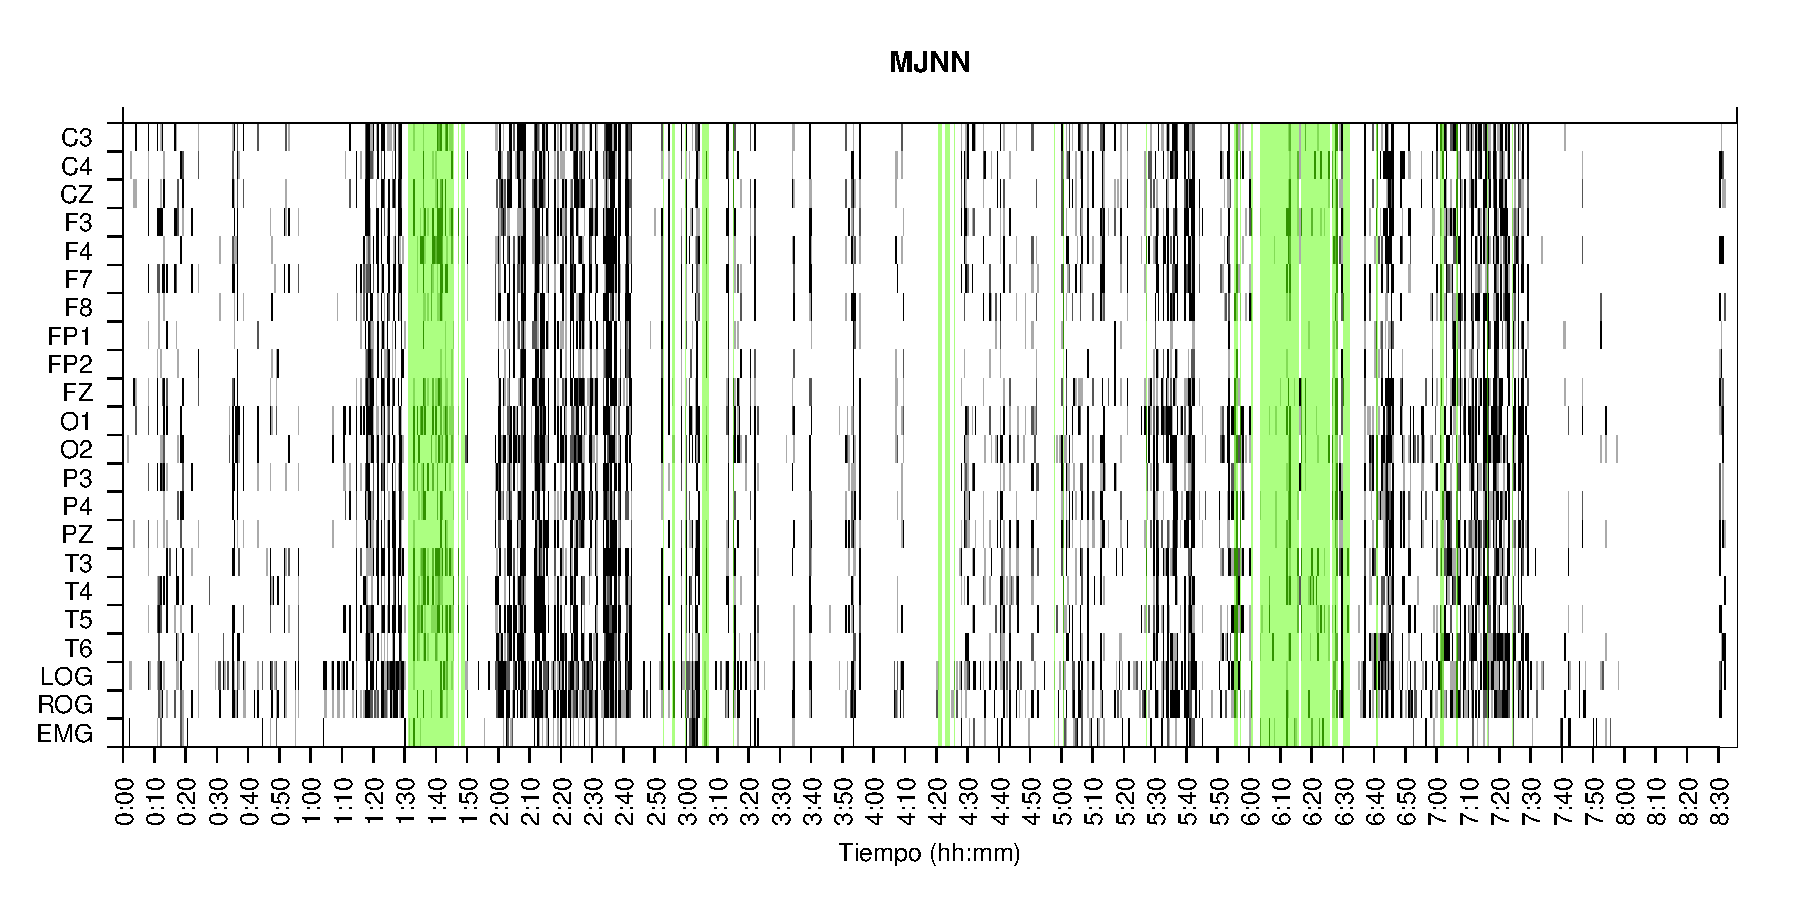
\includegraphics[width=\textwidth]{MJNNVIGILOS_127_mor127_tot1032_esttotal.pdf} 
%            \caption{Total de \'epocas: 1032, \'epocas MOR: 127}
%            %\label{ejemplo1}
%        \end{figure}
%    \end{landscape}
%    \clearpage% Flush page
%}

%%%%%%%%%%%%%%%%%%%%%%%%%%%%%%%%%%%
%%%%%%%%%%%%%%%%%%%%%%%%%%%%%%%%%%%

%\section{Compilados gr\'aficos}
%
%\begin{SidewaysFigure}
%\centering
%\includegraphics[width=\linewidth]
%{./material_bonito170220/MJNNVIGILOS_127_mor127_tot1032_est_total.pdf} 
%\caption{Sujeto: MJNN | Total \'epocas: 1032 | \'Epocas MOR: 127}
%%\label{primera}
%\end{SidewaysFigure}
%\begin{SidewaysFigure}
%\centering
%\includegraphics[width=\linewidth]
%{./material_bonito170220/MJNNVIGILOS_127_mor127_tot127_est_mor.pdf} 
%\caption{Sujeto: MJNN | \'Epocas MOR: 127 | (\'Unicamente \'epocas MOR)}
%%\label{primera}
%\end{SidewaysFigure}
%
%\begin{figure}
%\centering
%\includegraphics[width=\linewidth]
%{./material_bonito170220/porcentaje_bis/MJNNVIGILOS_127_1032_1_bar_porcentaje.pdf} 
%\caption{Sujeto: MJNN | Porcentaje de \'epocas \textit{posiblemente estacionarias}}
%\end{figure}
%
%%%%%%%%%%%%%%%%%%%%%%%%%%%%%%%%%%%%
%%%%%%%%%%%%%%%%%%%%%%%%%%%%%%%%%%%%
%
%\begin{SidewaysFigure}
%\centering
%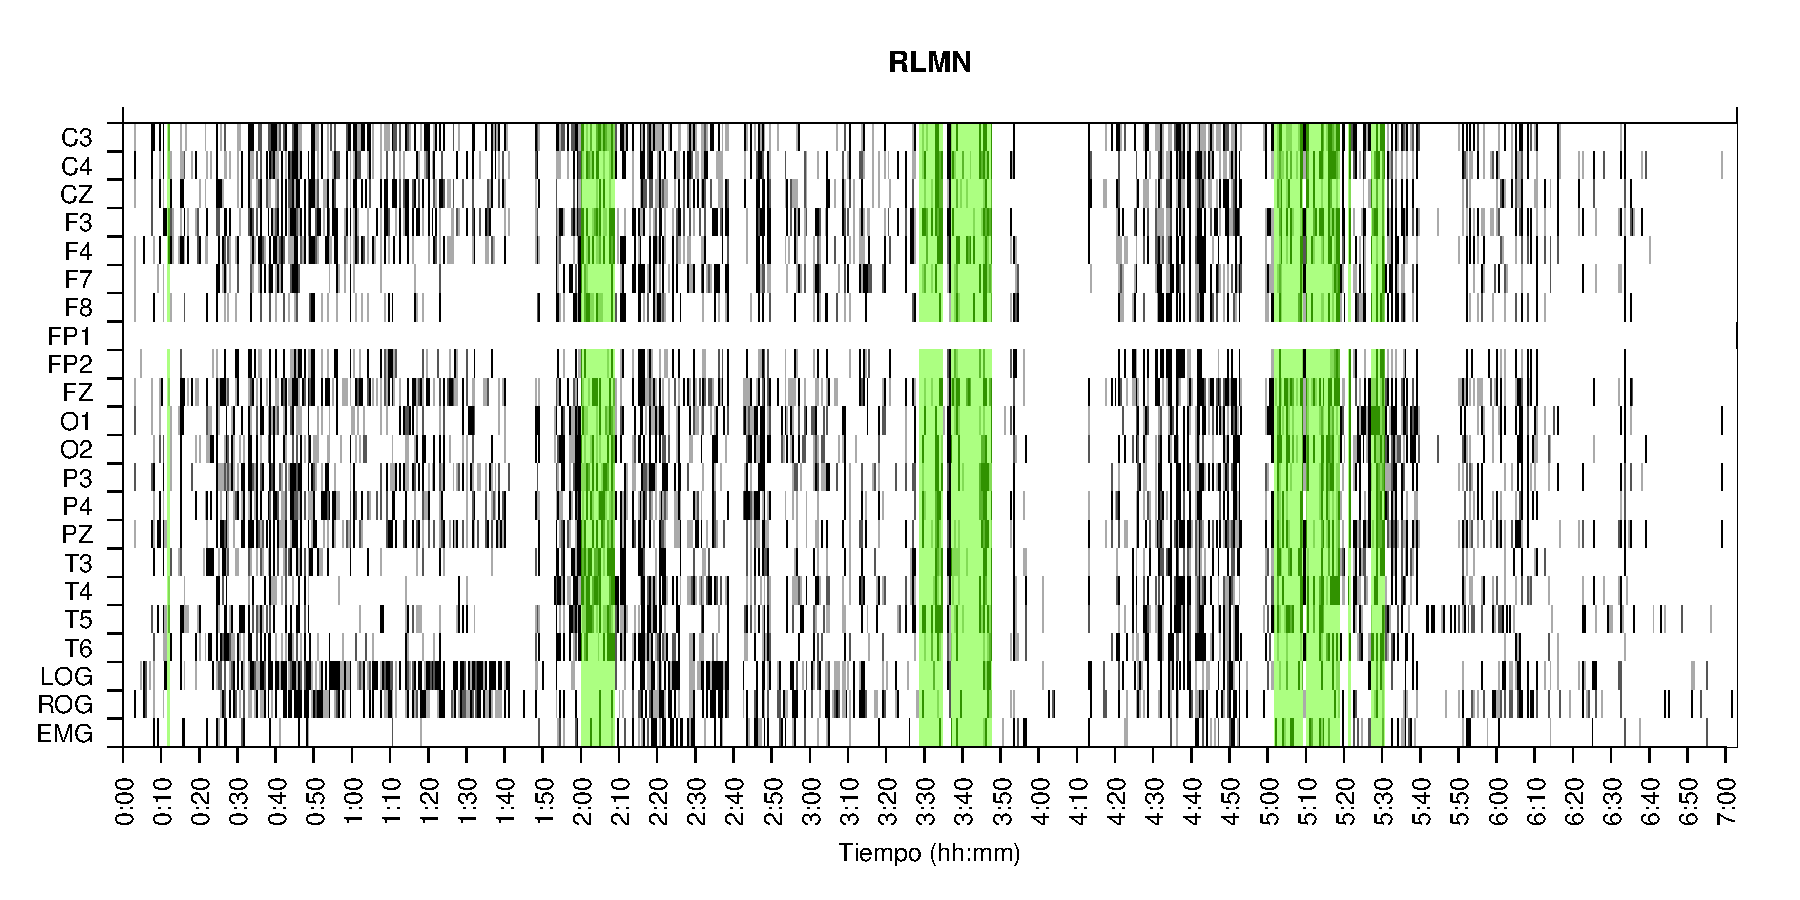
\includegraphics[width=\linewidth]{./material_bonito170220/RLMN10SUE_99_mor99_tot846_est_total.pdf} 
%\caption{Sujeto: RLMN | Total \'epocas: 846 | \'Epocas MOR: 99}
%%\label{primera}
%\end{SidewaysFigure}
%\begin{SidewaysFigure}
%\centering
%\includegraphics[width=\linewidth]
%{./material_bonito170220/RLMN10SUE_99_mor99_tot99_est_mor.pdf} 
%\caption{Sujeto: RLMN | \'Epocas MOR: 99 | (\'Unicamente \'epocas MOR)}
%%\label{primera}
%\end{SidewaysFigure}
%
%\begin{figure}
%\centering
%\includegraphics[width=\linewidth]
%{./material_bonito170220/porcentaje_bis/RLMN10SUE_99_846_1_bar_porcentaje.pdf} 
%\caption{Sujeto: RLMN | Porcentaje de \'epocas \textit{posiblemente estacionarias}}
%\end{figure}
%
%%%%%%%%%%%%%%%%%%%%%%%%%%%%%%%%%%%%
%%%%%%%%%%%%%%%%%%%%%%%%%%%%%%%%%%%%
%
%\begin{SidewaysFigure}
%\centering
%\includegraphics[width=\linewidth]
%{./material_bonito170220/JANASUE_103_mor103_tot907_est_total.pdf} 
%\caption{Sujeto: JANA | Total \'epocas: 907 | \'Epocas MOR: 103}
%%\label{primera}
%\end{SidewaysFigure}
%\begin{SidewaysFigure}
%\centering
%\includegraphics[width=\linewidth]
%{./material_bonito170220/JANASUE_103_mor103_tot103_est_mor.pdf} 
%\caption{Sujeto: JANA | \'Epocas MOR: 103 | (\'Unicamente \'epocas MOR)}
%%\label{primera}
%\end{SidewaysFigure}
%
%\begin{figure}
%\centering
%\includegraphics[width=\linewidth]
%{./material_bonito170220/porcentaje_bis/JANASUE_103_907_1_bar_porcentaje.pdf} 
%\caption{Sujeto: JANA | Porcentaje de \'epocas \textit{posiblemente estacionarias}}
%\end{figure}
%
%%%%%%%%%%%%%%%%%%%%%%%%%%%%%%%%%%%%
%%%%%%%%%%%%%%%%%%%%%%%%%%%%%%%%%%%%
%
%\begin{SidewaysFigure}
%\centering
%\includegraphics[width=\linewidth]
%{./material_bonito170220/CLMN10SUE_132_mor132_tot944_est_total.pdf} 
%\caption{Sujeto: CLMN | Total \'epocas: 944 | \'Epocas MOR: 132}
%%\label{primera}
%\end{SidewaysFigure}
%\begin{SidewaysFigure}
%\centering
%\includegraphics[width=\linewidth]
%{./material_bonito170220/CLMN10SUE_132_mor132_tot132_est_mor.pdf} 
%\caption{Sujeto: CLMN | \'Epocas MOR: 132 | (\'Unicamente \'epocas MOR)}
%%\label{primera}
%\end{SidewaysFigure}
%
%\begin{figure}
%\centering
%\includegraphics[width=\linewidth]
%{./material_bonito170220/porcentaje_bis/CLMN10SUE_132_944_1_bar_porcentaje.pdf} 
%\caption{Sujeto: CLMN | Porcentaje de \'epocas \textit{posiblemente estacionarias}}
%\end{figure}
%
%%%%%%%%%%%%%%%%%%%%%%%%%%%%%%%%%%%%
%%%%%%%%%%%%%%%%%%%%%%%%%%%%%%%%%%%%
%
%\begin{SidewaysFigure}
%\centering
%\includegraphics[width=\linewidth]
%{./material_bonito170220/CLMN10SUE_132_mor132_tot944_est_total.pdf} 
%\caption{Sujeto: JGMN | Total \'epocas: 1207 | \'Epocas MOR: 33}
%%\label{primera}
%\end{SidewaysFigure}
%\begin{SidewaysFigure}
%\centering
%\includegraphics[width=\linewidth]
%{./material_bonito170220/JGMN6SUE_33_mor33_tot33_est_mor.pdf} 
%\caption{Sujeto: CLMN | \'Epocas MOR: 33 | (\'Unicamente \'epocas MOR)}
%%\label{primera}
%\end{SidewaysFigure}
%
%\begin{figure}
%\centering
%\includegraphics[width=\linewidth]
%{./material_bonito170220/porcentaje_bis/JGMN6SUE_33_1207_1_bar_porcentaje.pdf} 
%\caption{Sujeto: JGMN | Porcentaje de \'epocas \textit{posiblemente estacionarias}}
%\end{figure}
%
%%%%%%%%%%%%%%%%%%%%%%%%%%%%%%%%%%%%
%%%%%%%%%%%%%%%%%%%%%%%%%%%%%%%%%%%%
%
%\begin{SidewaysFigure}
%\centering
%\includegraphics[width=\linewidth]
%{./material_bonito170220/RRMNS_114_mor114_tot1244_est_total_bis.pdf} 
%\caption{Sujeto: RRMN | Total \'epocas: 1244 | \'Epocas MOR: 114}
%%\label{primera}
%\end{SidewaysFigure}
%\begin{SidewaysFigure}
%\centering
%\includegraphics[width=\linewidth]
%{./material_bonito170220/RRMNS_114_mor114_tot114_est_mor_bis.pdf} 
%\caption{Sujeto: RRMN | \'Epocas MOR: 114 | (\'Unicamente \'epocas MOR)}
%%\label{primera}
%\end{SidewaysFigure}
%
%\begin{figure}
%\centering
%\includegraphics[width=\linewidth]
%{./material_bonito170220/porcentaje_bis/RRMNS_114_1244_1_bar_porcentaje.pdf} 
%\caption{Sujeto: RRMN | Porcentaje de \'epocas \textit{posiblemente estacionarias}}
%\end{figure}
%
%%%%%%%%%%%%%%%%%%%%%%%%%%%%%%%%%%%%
%%%%%%%%%%%%%%%%%%%%%%%%%%%%%%%%%%%%
%
%\begin{SidewaysFigure}
%\centering
%\includegraphics[width=\linewidth]
%{./material_bonito170220/VCNNS1_200_mor200_tot2584_est_total.pdf} 
%\caption{Sujeto: VCNN | Total \'epocas: 2586 | \'Epocas MOR: 200}
%%\label{primera}
%\end{SidewaysFigure}
%\begin{SidewaysFigure}
%\centering
%\includegraphics[width=\linewidth]
%{./material_bonito170220/VCNNS1_200_mor200_tot200_est_mor.pdf} 
%\caption{Sujeto: VCNN | \'Epocas MOR: 200 | (\'Unicamente \'epocas MOR)}
%%\label{primera}
%\end{SidewaysFigure}
%
%\begin{figure}
%\centering
%\includegraphics[width=\linewidth]
%{./material_bonito170220/porcentaje_bis/VCNNS1_200_2584_1_bar_porcentaje.pdf} 
%\caption{Sujeto: VCNN | Porcentaje de \'epocas \textit{posiblemente estacionarias}}
%\end{figure}
%
%%%%%%%%%%%%%%%%%%%%%%%%%%%%%%%%%%%%
%%%%%%%%%%%%%%%%%%%%%%%%%%%%%%%%%%%%
%
%\begin{SidewaysFigure}
%\centering
%\includegraphics[width=\linewidth]
%{./material_bonito170220/FGHSUE_22_mor22_tot405_est_total.pdf} 
%\caption{Sujeto: FGH | Total \'epocas: 405 | \'Epocas MOR: 22}
%%\label{primera}
%\end{SidewaysFigure}
%\begin{SidewaysFigure}
%\centering
%\includegraphics[width=\linewidth]
%{./material_bonito170220/FGHSUE_22_mor22_tot22_est_mor.pdf} 
%\caption{Sujeto: FGH | \'Epocas MOR: 22 | (\'Unicamente \'epocas MOR)}
%%\label{primera}
%\end{SidewaysFigure}
%
%\begin{figure}
%\centering
%\includegraphics[width=\linewidth]
%{./material_bonito170220/porcentaje_bis/FGHSUE_22_405_1_bar_porcentaje.pdf} 
%\caption{Sujeto: FGH | Porcentaje de \'epocas \textit{posiblemente estacionarias}}
%\end{figure}
%
%%%%%%%%%%%%%%%%%%%%%%%%%%%%%%%%%%%%
%%%%%%%%%%%%%%%%%%%%%%%%%%%%%%%%%%%%
%
%\begin{SidewaysFigure}
%\centering
%\includegraphics[width=\linewidth]
%{./material_bonito170220/GH24031950SUENO_267_mor267_tot3281_est_total.pdf} 
%\caption{Sujeto: GURM | Total \'epocas: 3281 | \'Epocas MOR: 267}
%%\label{primera}
%\end{SidewaysFigure}
%\begin{SidewaysFigure}
%\centering
%\includegraphics[width=\linewidth]
%{./material_bonito170220/GH24031950SUENO_267_mor267_tot267_est_mor.pdf} 
%\caption{Sujeto: GURM | \'Epocas MOR: 267 | (\'Unicamente \'epocas MOR)}
%%\label{primera}
%\end{SidewaysFigure}
%
%\begin{figure}
%\centering
%\includegraphics[width=\linewidth]
%{./material_bonito170220/porcentaje_bis/GH24031950SUENO_267_3281_1_bar_porcentaje.pdf} 
%\caption{Sujeto: GURM | Porcentaje de \'epocas \textit{posiblemente estacionarias}}
%\end{figure}

%%%%%%%%%%%%%%%%%%%%%%%%%%%%%%%%%%%
%%%%%%%%%%%%%%%%%%%%%%%%%%%%%%%%%%%

%%%%%%%%%%%%%%%%%%%%%%%%%%%%%%%%%%%%%%%%%%%%%%%%%%%%%%%%%%%%%%%%%%%%%%%%%%%%%%%%%%%%%%%%%%%%%%%%%%%
%%%%%%%%%%%%%%%%%%%%%%%%%%%%%%%%%%%%%%%%%%%%%%%%%%%%%%%%%%%%%%%%%%%%%%%%%%%%%%%%%%%%%%%%%%%%%%%%%%%